% Template for Cogsci submission with R Markdown

% Stuff changed from original Markdown PLOS Template
\documentclass[10pt, letterpaper]{article}

\usepackage{cogsci}
\usepackage{pslatex}
\usepackage{float}
\usepackage{caption}

% amsmath package, useful for mathematical formulas
\usepackage{amsmath}

% amssymb package, useful for mathematical symbols
\usepackage{amssymb}

% hyperref package, useful for hyperlinks
\usepackage{hyperref}

% graphicx package, useful for including eps and pdf graphics
% include graphics with the command \includegraphics
\usepackage{graphicx}

% Sweave(-like)
\usepackage{fancyvrb}
\DefineVerbatimEnvironment{Sinput}{Verbatim}{fontshape=sl}
\DefineVerbatimEnvironment{Soutput}{Verbatim}{}
\DefineVerbatimEnvironment{Scode}{Verbatim}{fontshape=sl}
\newenvironment{Schunk}{}{}
\DefineVerbatimEnvironment{Code}{Verbatim}{}
\DefineVerbatimEnvironment{CodeInput}{Verbatim}{fontshape=sl}
\DefineVerbatimEnvironment{CodeOutput}{Verbatim}{}
\newenvironment{CodeChunk}{}{}

% cite package, to clean up citations in the main text. Do not remove.
\usepackage{apacite}

% KM added 1/4/18 to allow control of blind submission


\usepackage{color}

% Use doublespacing - comment out for single spacing
%\usepackage{setspace}
%\doublespacing


% % Text layout
% \topmargin 0.0cm
% \oddsidemargin 0.5cm
% \evensidemargin 0.5cm
% \textwidth 16cm
% \textheight 21cm

\title{Generalizing from individuals to populations:\\
Hierarchical inference supports convention formation on networks}


\author{{\large \bf Morton Ann Gernsbacher (MAG@Macc.Wisc.Edu)} \\ Department of Psychology, 1202 W. Johnson Street \\ Madison, WI 53706 USA \AND {\large \bf Sharon J.~Derry (SDJ@Macc.Wisc.Edu)} \\ Department of Educational Psychology, 1025 W. Johnson Street \\ Madison, WI 53706 USA}

\begin{document}

\maketitle

\begin{abstract}
Linguistic conventions allow us to communicate efficiently even with
novel members of our community. At the same time, much of our intended
meaning is partner-specific. Exactly how do agents make the inferential
leap to community-wide expectations from their experiences with specific
partners? We propose a hierarchical Bayesian model that explains how
partner-specific pacts may spread through a network and present
simulations of how speakers and listeners generalize meanings across
partners. To evalute these predictions, we collected experimental data
showing how people conventionalize referring expressions in a series of
interactive reference games with different partners in a small
community. These results suggest that local partner-specific learning is
not only compatible with global convention formation but may facilitate
it when coupled with a powerful hierachical inductive mechanism.

\textbf{Keywords:}
convention; generalization;
\end{abstract}

To communicate successfully, speakers and listeners must share a common
system of semantic meaning in the language they are using. These
meanings are \emph{conventional} in the sense that they are sustained by
the expectations each person has about others (Bicchieri, 2006; Lewis,
1969). A key property of linguistic conventions is that they hold over
an entire community of speakers, allowing us to communicate efficiently
even with people we've never met before. But exactly how do we make the
inferential leap to community-wide expectations from our experiences
with specific partners? Grounding collective convention formation in
individual cognition requires an explicit \emph{theory of
generalization} capturing how people transfer what they have learned
from one partner to the next.

One influential theory is that speakers simply ignore the identity of
different partners and update a single monolithic representation after
every interaction (Baronchelli, 2018; Barr, 2004; Steels, 1995; Young,
2015). We call this a \emph{complete-pooling} theory because data from
each partner is collapsed into an undifferentiated pool of evidence
(Gelman \& Hill, 2006). Complete-pooling models have been remarkably
successful at predicting collective behavior on networks, but have
typically been evaluated only in settings where anonymity is enforced.
For example, Centola \& Baronchelli (2015) asked how large networks of
participants coordinated on conventional names for novel faces. On each
trial, participants were paired with a random neighbor but were not
informed of that neighbor's identity, or even the total number of
different possible neighbors.

While complete-pooling may be appropriate for some everyday social
interactions, such as coordinating with anonymous drivers on the
highway, it is less tenable for everyday communicative settings.
Knowledge about a partner's identity is both available and relevant for
conversation (Eckert, 2012). Extensive evidence from psycholinguistics
has demonstrated the \emph{partner-specificity} of our language use
(Brennan \& Hanna, 2009; Clark, 1996). Because meaning is grounded in
the evolving `common ground' shared with each partner, meanings
established over a history of interaction with one partner are not
necessary transfered to other partners (Metzing \& Brennan, 2003;
Wilkes-Gibbs \& Clark, 1992). Partner-specificity thus poses clear
problems for complete-pooling theories but can be easily explained by
another simple model, where agents maintain separate expectations about
meaning for each partner. We call this a \emph{no-pooling} model. The
problem with no-pooling, of course, is that agents are forced to start
from scratch with each partner. Community-level expectations never get
off the ground.

What theory of generalization, then, can explain partner-specific
meaning but also allow conventions to spread through communities? We
propose a \emph{partial-pooling} account that offers a compromise
between these extremes. Unlike complete-pooling and no-pooling models,
we propose that beliefs about meaning have hierarchical structure. That
is, the meanings used by different partners are expected to be drawn
from a shared community-wide distribution but are also allowed to differ
from one another in systematic, partner-specific ways. This structure
provides an inductive pathway for abstract population-level expectations
to be distilled from partner-specific experience (see also Kleinschmidt
\& Jaeger, 2015; Tenenbaum, Kemp, Griffiths, \& Goodman, 2011).

We begin by formalizing this account in a probabilistic model of
communication and presenting several simulations of listener and speaker
behavior within and across partners. Next, we test the qualitative
predictions of this model in a behavioral experiment. Participants were
paired for a series of extended reference games with each neighbor in
small networks. Our results showed signatures of \emph{ad hoc}
convention formation within dyads, but also gradual generalization of
these local pacts across subsequent partners as the network converged.
Taken together, these results suggest that local partner-specific
learning is not only compatible with global convention formation but may
facilitate it when coupled with a powerful hierachical inductive
mechanism.

\hypertarget{a-hierarchical-bayesian-model-of-convention}{%
\section{A hierarchical Bayesian model of
convention}\label{a-hierarchical-bayesian-model-of-convention}}

\begin{CodeChunk}
\begin{figure}[t]

{\centering 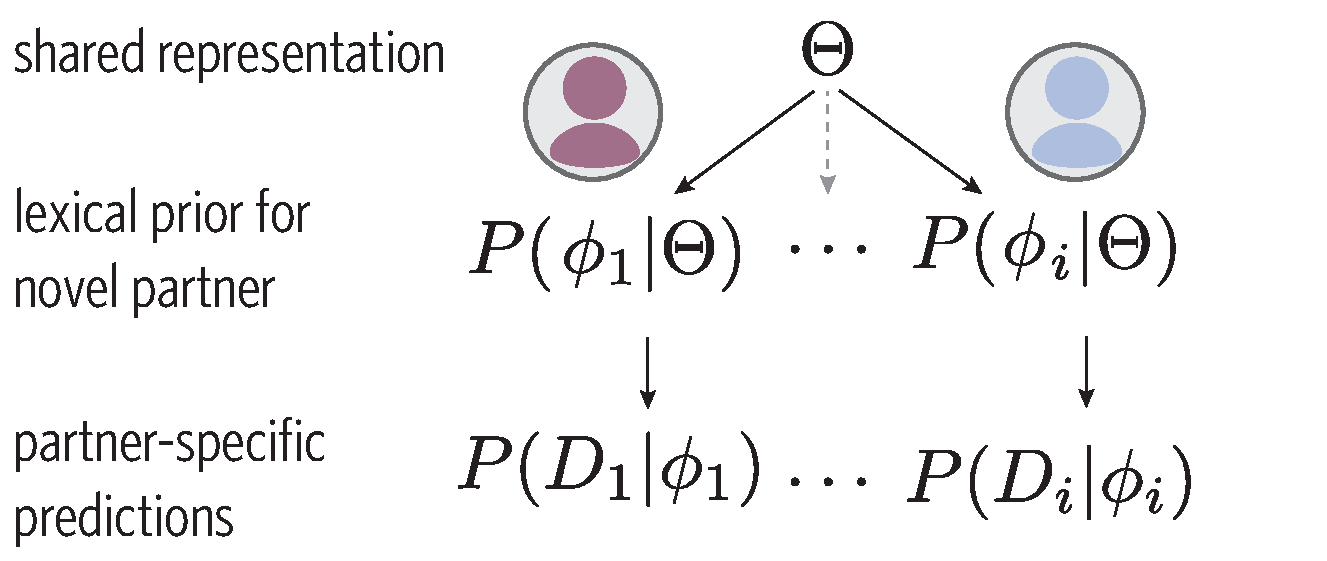
\includegraphics[width=225px]{figs/task1_model} 

}

\caption{\label{fig:task1model} Schematic of hierachical Bayesian model.}\label{fig:model_schematic}
\end{figure}
\end{CodeChunk}

In this section, we provide an explicit computational account of the
cognitive mechanisms supporting the balance between community-level
stability and partner-specific flexibility. Specifically, we show how
the dyadic convention formation model of Hawkins, Frank, \& Goodman
(2017) can be extended with a principled mechanism for generalization
across multiple partners. This model begins with the idea that knowledge
about meanings can be represented probabilistically: agents have
uncertainty about what lexical meaning their current partner is using
(Bergen, Levy, \& Goodman, 2016). In our hierarchical model, this
lexical uncertainty is represented by a multi-level prior.

At the highest level of the hierarchy is a \emph{community-level}
variable \(\Theta\) parameterizing the agent's \emph{partner-specific}
expectations \(P(\phi_{k} | \Theta)\), where \(\phi_k\) represents the
latent system of meanings used by partner \(k\) (see Fig.
\ref{fig:task1model}). Given observations \(D_k\) from repeated
communicative interactions with a specific partner \(i\), the agent
updates their beliefs about the latent system of meaning using Bayes
rule: \begin{equation}
\begin{array}{rcl}
P(\phi_k, \Theta | D_k)  & \propto &  P(D_k | \phi_k, \Theta) P(\phi_k, \Theta) \\
                           & =   & P(D_k | \phi_k) P(\phi_k | \Theta) P(\Theta)
\end{array}
\end{equation}

This inference decomposes the problem of partner-specific learning into
two terms, a prior term \(P(\phi_k | \Theta)P(\Theta)\) and a likelihood
term \(P(D_k | \phi_k)\). The prior captures the idea that different
partners will share some aspects of meaning in common. In the absence of
strong information about partner-specific language use departing from
this common structure, the agent ought to be regularized toward
generalizable knowledge of their community's conventions (Davidson,
1986). The likelihood represents predictions about how a partner using a
particular system of meaning will use language.

This joint posterior over meanings has two consequences for convention
formation. First, it allows agents to maintain partner-specific
expectations \(\phi_k\) by marginalizing over community-level
uncertainty: \begin{equation}
P(\phi_k | D_k) = \int_{\Theta}P(D_k | \phi_k) P(\phi_k | \Theta) P(\Theta)  d\Theta
\end{equation} Second, the hierarchical structure provides an inductive
pathway for data to inform beliefs about community-wide conventions.
Agents update their beliefs about \(\Theta\) by marginalizing over data
accumulated from different partners: \begin{equation}
P(\Theta | D) = P(\Theta) \int_{\phi} P(D_k | \phi_k) P(\phi_k | \Theta) d\phi
\end{equation} where \(D = \bigcup_{k=1}^N D_k\),
\(\phi = \phi_1 \times \dots \times \phi_N\), and \(N\) is the number of
partners previous encountered. Given weak community-level expectations
about \(\Theta\), a particular partner's behavior may at first be more
parsimoniously explained with a partner-specific model. After multiple
partners are inferred to have a similar system of meaning, however,
beliefs about \(\Theta\) shift to represent this abstracted knowledge:
it becomes more likely that a novel partner will share it as well. This
transfer is sometimes referred to as a ``sharing of strength'' or
``partial pooling'' (Gelman \& Hill, 2006) because abstractions are
smoothly integrated with domain-specific detail depending on the data
available.

\hypertarget{model-simulations}{%
\subsection{Model simulations}\label{model-simulations}}

\begin{CodeChunk}
\begin{figure*}[t!]

{\centering \includegraphics{figs/model_results-1} 

}

\caption{\label{fig:simulations} Model predictions across a series of different partners.}\label{fig:model_results}
\end{figure*}
\end{CodeChunk}

We investigate the qualitative predictions of this model under three
increasingly complex scenarios. In all of these scenarios, speaker and
listener agents play a reference game with a set of two objects
\(\{o_1, o_2\}\). On each trial, one of these objects is designated for
the speaker as the \emph{target}. They must select from a set of
utterance \(\{u_0, \dots, u_j\}\) to convey the identity of the target
to the listener. Upon hearing this utterance, the listener selects which
of the objects they believe to be the target and then receives feedback
about the true target. The resulting data \(D_k\) from an interaction
with partner \(k\) thus consists of utterance-object pairs
\(\{(u, o)_t\}\) for each trial \(t\).

Given this reference game setting, we can now explicitly specify the
likelihood and prior terms. We consider a likelihood given by the
Rational Speech Act (RSA) framework, which formalizes the Gricean
assumption of cooperativity (Franke \& Jäger, 2016; Goodman \& Frank,
2016). A pragmatic speaker \(S_1\) attempts to trade off informativity
against the cost of producing an utterance, while a pragmatic listener
\(L_1\) inverts their model of the speaker to infer the intended target.
The chain of recursive social reasoning grounds out in a
\emph{literal listener} \(L_0\), who identifies an intended meaning from
their content-addressible memory for lexical items
\(\mathcal{L}_{\phi_k}\). This model can be formally specified as
follows: \[
\begin{array}{rcl}
L_0(o | u, \phi_k) &\propto  & \exp\{\mathcal{L}_{\phi_k}(u,o)\} \\
S_1(u | o, \phi_k) &\propto &  \exp\{w_I \cdot \log L_0(o | u, \phi_k) - w_C \cdot \textrm{cost}(u)\}   \\
L_1(o | u, \phi_k) &\propto  & S_1(u | o, \phi_k) P(o) 
\end{array}
\] where \(w_I\) and \(w_C\) are free parameters controlling the
relative weights on the informativity and cost term, respectively. We
define \(P(D_k | \phi_k)\) as the probability of the data under a
pragmatic listener \(L_1\). We also use this RSA model to simulate the
behavior of uncertain speakers \(S\) and listeners \(L\). Utterances and
object selections are sampled from the posterior predictive,
marginalizing over lexical uncertainty.

Finally, we must specify the form of the lexical prior and a method to
perform inference in this model. We assume \(\Theta\) is a matrix with
an entry for each utterance-object pair \((u_i, o_j)\), and use
independent Gaussian distributions for each \(\Theta_{ij} \in \Theta\)
as a hyper-prior. We then centered our partner-specific prior
\(\phi_{ij} \in \phi\) at the shared value for a particular partner:
\[\begin{array}{rcl}
P(\Theta_{ij}) & \sim & \mathcal{N}(0, 1)\\
P(\phi_{ij} | \Theta_{ij}) & \sim & \mathcal{N}(\Theta_{ij}, 1)
\end{array}\] Note that the variances chosen in these priors represent
assumptions about how far partner-specific priors can drift from the
community-wide value.

For all simulations, we used variational inference (VI; Ranganath,
Gerrish, \& Blei, 2013) to perform inference. Variational methods
transform probabilistic inference problems into optimization problems by
approximating the true posterior with a parameterized family.
Specifically, we make a \emph{mean-field} approximation and assume that
the full posterior can be factored into independent Gaussians for each
random variable in the lexicon. We then optimize the parameters of these
posterior Gaussians by minimizing the evidence lower bound (ELBO)
objective (see Murphy, 2012 for more details). Variational inference
allows us to amortize inference as additional data is observed. We run
50,000 steps of gradient descent on the first observation to obtain a
posterior, compute the agent's marginal prediction for the next
observation by taking the expectation over 50,000 samples from the
posterior predictive, then continue running gradient descent on the same
parameters after adding the new observation in the data.

\hypertarget{simulation-1-listener-accuracy-across-partners}{%
\subsubsection{Simulation 1: Listener accuracy across
partners}\label{simulation-1-listener-accuracy-across-partners}}

The key predictions of our model concern the pattern of generalization
across partners. In our first simulation, we consider the
partner-specificity of a listener's expectations about which object is
being referred to. To observe the model's behavior in the simplest case,
we assume the speaker has a vocabulary of two utterances
\(\{u_1, u_2\}\) and feed the model the same utterance-object pair
(\(\{o_1, u_1\}\)) on every trial. Instead of presenting this stream of
data from a single partner, or randomly choosing a different partner on
every trial, we swap in a new partner every block of 4 trials.

Our simulation results are shown in Fig. \ref{fig:simulations}A. The
listener begins at chance due to its uninformative prior, but after
observing several trial of evidence from the same partner, it learns to
choose the true target with high accuracy. When a new partner is
introduced, it reverts nearly to its original state. Because of the
hierarchical structure of its lexical expectations, it was ambiguous
whether the evidence from the first partner was idiosyncratic or due to
shared structure. After adapting to multiple partners, however, we find
that it has stronger initial expectations by its fourth partner. Thus,
expectations about what an individual partner means have gradually been
incorporated into community-level expectations.

\begin{CodeChunk}
\begin{figure*}[t!]

{\centering 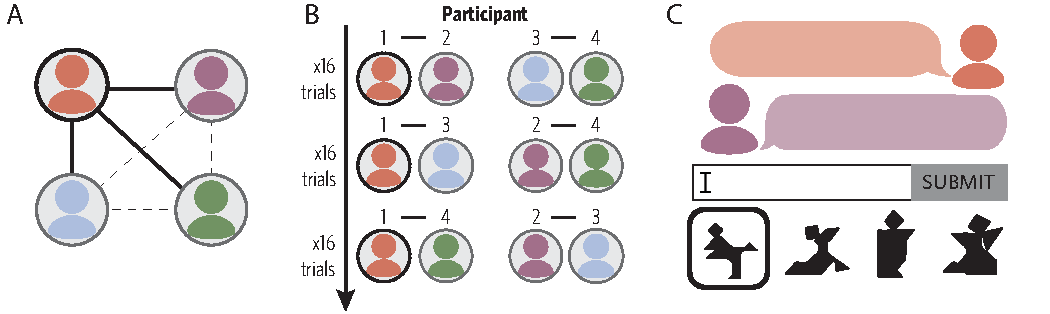
\includegraphics{figs/design} 

}

\caption{\label{fig:task1_display} Experimental design. (A) Participants were placed in fully-connected networks of 4 and (B) played repeated reference games with each partner.}\label{fig:task_display}
\end{figure*}
\end{CodeChunk}

\hypertarget{simulation-2-speaker-utterance-length-across-partners}{%
\subsubsection{Simulation 2: Speaker utterance length across
partners}\label{simulation-2-speaker-utterance-length-across-partners}}

Next, we show that our model accounts for the \emph{partner-specificity}
of the speaker's referring expressions (Wilkes-Gibbs \& Clark, 1992). We
supplement the utterance space with multi-word utterances built from a
set of four primitives: \(\{u_1, u_2, u_3, u_4\}\). Under our model,
speakers revert back to a longer description with a novel partner
because evidence from a single listener is relatively uninformative
about the community-level prior. After interacting with enough partners
in a tight-knit community, speakers should become increasingly confident
that labels are not simply idiosyncratic features of a particular
partner's lexicon but are shared across the entire community. In other
words, the partner-specific expectations agents form within an
interaction to solve novel communication problems gradually generalize
to community-wide expectations as they gain additional evidence of the
latent population-level distribution from which different partners are
sampled. These expectations manifest in an increasing willingness to use
shorter labels with novel partners (Fig. \ref{fig:simulations}B).

\hypertarget{simulation-3-network-convergence}{%
\subsubsection{Simulation 3: Network
convergence}\label{simulation-3-network-convergence}}

The first two simulations presented a single agent with a fixed sequence
of data to understand its gradient of generalization within and across
partners. Here, we test the consequences of the proposed hierarchical
inference scheme for a network of interacting agents. How does the
network as a whole coordinate? Do agents come to share a similar
\(\Theta\), suggesting that community-wide conventions have formed? We
used a round-robin scheme to schedule four agents into three blocks of
interaction, with agents taking turns in the speaker and listener roles.
From each individual agent's perspective, this experiment is identical
to the earlier simulation (i.e.~a series of 3 partners). Because all
agents are not learning from the others, however, the network as a whole
faces a coordination problem. For example, in the first block, agent 1
and 2 may coordinate on using \(u_1\) while agent 3 and 4 coordinate no
using \(u_2\). Once they swap partners, they must re-negotiate this
potential miscoordination. We find that the network as a whole gradually
aligns (Fig. \ref{fig:simulations}C).

\hypertarget{behavioral-experiment-convention-formation-on-a-network}{%
\section{Behavioral experiment: ~Convention formation on a
network}\label{behavioral-experiment-convention-formation-on-a-network}}

To evaluate these qualitative predictions, we designed a communication
experiment on a small network. Rather than anonymizing partners, we
divided the experiment into blocks of contiguous interaction with stable
partners (see Fay, Garrod, Roberts, \& Swoboda, 2010; Garrod \& Doherty,
1994 for similar designs). Each block was a full repeated reference
game, where participants had to coordinate on an \emph{ad hoc}
convention, or \emph{pact}, for how to refer to reoccuring target
objects with their partner (Brennan \& Clark, 1996).

While it has been frequently observed that messages reduce in length
across repetitions as common ground is built a single partner (Krauss \&
Weinheimer, 1964), and sharply revert back to longer utterances when a
new partner is introduced (Wilkes-Gibbs \& Clark, 1992), the key
empirical predictions distinguishing our model from alternatives concern
behavior across partner boundaries. Complete-pooling accounts predict no
change in the number of words when a new partner is introduced and are
thus inconsistent even with the results of Wilkes-Gibbs \& Clark (1992).
No-pooling accounts predict that roughly the same initial description
length will re-occur with every subsequent interlocutor. Contrary to
either of these extremes, our hierarchical Bayesian model predicts that
description length will increase at partner boundaries but that the
initial length will decrease incrementally over successive interactions:
after each partner, agents should be more willing to transfer
expectations from one partner to another in their community.

\hypertarget{methods}{%
\subsection{Methods}\label{methods}}

\hypertarget{participants}{%
\subsubsection{Participants}\label{participants}}

We recruited 92 participants from Amazon Mechanical Turk to play an
interactive, natural-language reference game implemented with the
Dallinger platform\footnote{http://docs.dallinger.io/}.

\hypertarget{stimuli-and-procedure}{%
\subsubsection{Stimuli and procedure}\label{stimuli-and-procedure}}

Participants were randomly assigned to one of 23 fully-connected
four-person communities of `neighbors' (Fig. \ref{fig:task1_display}A)
and paired with each of their three neighbors in a series of real-time,
natural-language reference games. Pairings were determined by a
round-robin schedule (Fig. \ref{fig:task1_display}B). Each network was
randomly assigned one of three distinct sets of four abstract tangram
stimuli taken from Clark and Wilkes-Gibbs (1986, see Fig.
\ref{fig:task1_display}C). These stimuli were chosen because
participants do not already have strong pre-existing lexical conventions
for how to refer to them (unlike photographs of common objects), but
they are structured enough to support many possible descriptions (unlike
images of white noise).

On each trial, one of these four shapes was highlighted as the
\emph{target object} for the ``speaker'' who was instructed to use a
chatbox to communicate the identity of this object to their partner, the
``listener''. The listener could reply freely through the chatbox but
was asked to ultimately make a selection from the array. Finally, both
participants in a pair were given full feedback on each trial about
their partner's choice and received bonus payment for each correct
response.

The trial sequence for a given partner was constructed so that each of
the four targets appeared once per block, for four continuous blocks.
After completing sixteen trials with one partner, participants were
introduced to their next partner and asked to play the repeated
reference game again with the same four objects. This process repeated
until each participant had partnered with all three neighbors.
Participants in a network were assigned distinct avatars to emphasize
that participants were speaking to the same partner for an extended
period. Because some pairs within the network took longer than others to
complete the trial sequence, we sent participants to a temporary waiting
room if their next partner was not yet ready.

\begin{CodeChunk}
\begin{figure*}[t!]

{\centering \includegraphics{figs/reduction-1} 

}

\caption{\label{fig:results}(A)Increase in accuracy across partners, (B) reduction in number of words across partners, (C) network convergence.}\label{fig:reduction}
\end{figure*}
\end{CodeChunk}

\hypertarget{results}{%
\subsection{Results}\label{results}}

We evaluate our model's predictions on the same three metrics we
reported in the simulations: accuracy, utterance length, and network
convergence.

\hypertarget{listener-accuracy}{%
\subsubsection{Listener accuracy}\label{listener-accuracy}}

TODO. (see Fig. \ref{fig:results}A)

\hypertarget{speaker-utterance-length}{%
\subsubsection{Speaker utterance
length}\label{speaker-utterance-length}}

The mean number of words used per description is a standard measure of
coding efficiency in reference games. We tested predictions using a
mixed-effects regression of partner number and repetition block number
on the length of the speaker's description. We included a random-effect
structure including item-effects at the object and speaker level.
\aeg{by-item, by-subject slopes and intercepts for partner \# and repetition \#?}
We find a positive jump in description length across partner-boundaries
overall, t(91) = 3.7, p \textless{} 0.001, indicating sensitivity to
different partners, but a successive incremental decrease in the lengths
of these initial descriptions, t(79.2) = -6.8, p \textless{} 0.001 (Fig.
\ref{fig:results}B). \aeg{why t-test and not intercepts?}

\hypertarget{network-convergence}{%
\subsubsection{Network convergence}\label{network-convergence}}

TODO. (Fig. \ref{fig:results}C).

\hypertarget{discussion}{%
\section{Discussion}\label{discussion}}

In other words, we suggest that conventional meanings result from agents
solving a meta-learning problem, adapting to each partner along the way.

\begin{enumerate}
\def\labelenumi{\arabic{enumi}.}
\item
  Other advantages of hierarchical model. e.g.~it's more robust to
  deviations than complete-pooling; if we have a lot of interactions
  with idiosyncratic speakers (e.g.~children), we don't replace our
  conventional community-level expectations. But agent-based models with
  a memory window or single representation predict this. Also there are
  other kinds of partner-specific information that may need to be
  tracked (e.g.~visual access/knowledge, e.g.~if you know someone is an
  expert in an area).
\item
  Possible connection to memory mechanisms: partners as contexts that
  get reinstated ({\textbf{???}}; Horton \& Gerrig, 2016), and
  \aeg{I'm not wild about "looking up" meaning in a "parameterized lexicon", preferring "a literal listener, L0, who identifies an intended meaning from their content-addressible memory which may include information about individual speakers or subgroups of speakers as well as phonological, contextual, and interpretative information" but for current purposes, fine!}
\item
  Suggest ideas about different communities and code-switching as
  targets of future work. e.g.~The current work captures and quantifies
  incremental convergence within communities of 4 unfamiliar English
  speakers towards a set of shared language conventions. We recognize
  that real-world communities are more complex than this, however, as
  each speaker takes part in a number of subcommunities which vary in
  size and overlap. For example, we use largely overlapping but
  partially distinct conventions depending on whether we are
  communicating with psychologists, friends from high school,
  bilinguals, or children, and we comprehend certain conventions that we
  do not use ourselves. To model the full scale of an individual's
  network of communities, social factors and cues are required. A
  strength of the hierachical Bayesian framework is that knowledge about
  these communities can be learned and represented in the generative
  model of a speaker ({\textbf{???}}). The current work suggests that
  hierarchical generalization may be a foundational cognitive building
  block for establishing conventionality at the group level while
  maintaining flexibility within interactions.
\end{enumerate}

\hypertarget{references}{%
\section{References}\label{references}}

\setlength{\parindent}{-0.1in} 
\setlength{\leftskip}{0.125in}

\noindent

\hypertarget{refs}{}
\leavevmode\hypertarget{ref-baronchelli_emergence_2018}{}%
Baronchelli, A. (2018). The Emergence of Consensus. \emph{Royal Society
Open Science}, \emph{5}(2).

\leavevmode\hypertarget{ref-barr_establishing_2004}{}%
Barr, D. J. (2004). Establishing conventional communication systems: Is
common knowledge necessary? \emph{Cognitive Science}, \emph{28}(6),
937--962.

\leavevmode\hypertarget{ref-bergen_pragmatic_2016}{}%
Bergen, L., Levy, R., \& Goodman, N. (2016). Pragmatic reasoning through
semantic inference. \emph{Semantics and Pragmatics}, \emph{9}(20).

\leavevmode\hypertarget{ref-bicchieri_grammar_2006}{}%
Bicchieri, C. (2006). \emph{The grammar of society: The nature and
dynamics of social norms}. Cambridge University Press.

\leavevmode\hypertarget{ref-BrennanClark96_ConceptualPactsConversation}{}%
Brennan, S. E., \& Clark, H. H. (1996). Conceptual pacts and lexical
choice in conversation. \emph{Journal of Experimental Psychology:
Learning, Memory, and Cognition}, \emph{22}(6), 1482.

\leavevmode\hypertarget{ref-brennan_partner-specific_2009}{}%
Brennan, S. E., \& Hanna, J. E. (2009). Partner-specific adaptation in
dialog. \emph{Topics in Cognitive Science}, \emph{1}(2).

\leavevmode\hypertarget{ref-centola_spontaneous_2015}{}%
Centola, D., \& Baronchelli, A. (2015). The spontaneous emergence of
conventions: An experimental study of cultural evolution.
\emph{Proceedings of the National Academy of Sciences}, \emph{112}(7),
1989--1994.

\leavevmode\hypertarget{ref-clark_using_1996}{}%
Clark, H. H. (1996). \emph{Using language}. Cambridge university press
Cambridge.

\leavevmode\hypertarget{ref-clark_referring_1986}{}%
Clark, H. H., \& Wilkes-Gibbs, D. (1986). Referring as a collaborative
process. \emph{Cognition}, \emph{22}(1), 1--39.

\leavevmode\hypertarget{ref-davidson_nice_1986}{}%
Davidson, D. (1986). A nice derangement of epitaphs. \emph{Philosophical
Grounds of Rationality: Intentions, Categories, Ends}, \emph{4},
157--174.

\leavevmode\hypertarget{ref-eckert_three_2012}{}%
Eckert, P. (2012). Three waves of variation study: The emergence of
meaning in the study of sociolinguistic variation. \emph{Annual Review
of Anthropology}, \emph{41}, 87--100.

\leavevmode\hypertarget{ref-fay_interactive_2010}{}%
Fay, N., Garrod, S., Roberts, L., \& Swoboda, N. (2010). The interactive
evolution of human communication systems. \emph{Cognitive Science},
\emph{34}(3).

\leavevmode\hypertarget{ref-FrankeJager16_ProbabilisticPragmatics}{}%
Franke, M., \& Jäger, G. (2016). Probabilistic pragmatics, or why Bayes'
rule is probably important for pragmatics. \emph{Zeitschrift Für
Sprachwissenschaft}, \emph{35}(1), 3--44.

\leavevmode\hypertarget{ref-garrod_conversation_1994}{}%
Garrod, S., \& Doherty, G. (1994). Conversation, co-ordination and
convention: An empirical investigation of how groups establish
linguistic conventions. \emph{Cognition}, \emph{53}(3).

\leavevmode\hypertarget{ref-gelman2006data}{}%
Gelman, A., \& Hill, J. (2006). \emph{Data analysis using regression and
multilevel/hierarchical models}. Cambridge university press.

\leavevmode\hypertarget{ref-GoodmanFrank16_RSATiCS}{}%
Goodman, N. D., \& Frank, M. C. (2016). Pragmatic language
interpretation as probabilistic inference. \emph{Trends in Cognitive
Sciences}, \emph{20}(11), 818--829.

\leavevmode\hypertarget{ref-hawkins_convention-formation_2017}{}%
Hawkins, R. X. D., Frank, M. C., \& Goodman, N. D. (2017).
Convention-formation in iterated reference games. In \emph{Proceedings
of the 39th annual meeting of the cognitive science society}.

\leavevmode\hypertarget{ref-horton_revisiting_2016}{}%
Horton, W. S., \& Gerrig, R. J. (2016). Revisiting the Memory-Based
Processing Approach to Common Ground. \emph{Topics in Cognitive
Science}.

\leavevmode\hypertarget{ref-KleinschmidtJaeger15_RobustSpeechPerception}{}%
Kleinschmidt, D. F., \& Jaeger, T. F. (2015). Robust speech perception:
Recognize the familiar, generalize to the similar, and adapt to the
novel. \emph{Psychological Review}, \emph{122}(2), 148.

\leavevmode\hypertarget{ref-krauss_changes_1964}{}%
Krauss, R. M., \& Weinheimer, S. (1964). Changes in reference phrases as
a function of frequency of usage in social interaction: A preliminary
study. \emph{Psychonomic Science}, \emph{1}(1-12), 113--114.

\leavevmode\hypertarget{ref-lewis_convention:_1969}{}%
Lewis, D. (1969). \emph{Convention: A philosophical study}. Harvard
University Press.

\leavevmode\hypertarget{ref-metzing_when_2003}{}%
Metzing, C., \& Brennan, S. E. (2003). When conceptual pacts are broken:
Partner-specific effects on the comprehension of referring expressions.
\emph{Journal of Memory and Language}, \emph{49}(2).

\leavevmode\hypertarget{ref-murphy2012machine}{}%
Murphy, K. P. (2012). \emph{Machine learning: A probabilistic
perspective}. MIT press.

\leavevmode\hypertarget{ref-RanganathGerrishBlei13_BlackBoxVariationalInference}{}%
Ranganath, R., Gerrish, S., \& Blei, D. M. (2013). Black box variational
inference. \emph{arXiv Preprint arXiv:1401.0118}.

\leavevmode\hypertarget{ref-steels_self-organizing_1995}{}%
Steels, L. (1995). A self-organizing spatial vocabulary.
\emph{Artificial Life}, \emph{2}(3), 319--332.

\leavevmode\hypertarget{ref-tenenbaum_how_2011}{}%
Tenenbaum, J. B., Kemp, C., Griffiths, T. L., \& Goodman, N. D. (2011).
How to grow a mind: Statistics, structure, and abstraction.
\emph{Science}, \emph{331}(6022), 1279--1285.

\leavevmode\hypertarget{ref-wilkes-gibbs_coordinating_1992}{}%
Wilkes-Gibbs, D., \& Clark, H. H. (1992). Coordinating beliefs in
conversation. \emph{Journal of Memory and Language}, \emph{31}(2),
183--194.

\leavevmode\hypertarget{ref-young_evolution_2015}{}%
Young, H. P. (2015). The Evolution of Social Norms. \emph{Annual Review
of Economics}, \emph{7}, 359--387.

\bibliographystyle{apacite}


\end{document}
